\documentclass{article}
\usepackage[margin=1in]{geometry}
\usepackage{amsmath}
\usepackage{amssymb}
\usepackage{listings}
\usepackage{graphicx}
\usepackage{color}
\usepackage{pdfpages}

\pagestyle{empty}

\graphicspath{{./}}
 
\definecolor{codegreen}{rgb}{0,0.6,0}
\definecolor{codegray}{rgb}{0.5,0.5,0.5}
\definecolor{codepurple}{rgb}{0.58,0,0.82}
\definecolor{backcolour}{rgb}{0.95,0.95,0.92}
 
\lstdefinestyle{mystyle}{
    backgroundcolor=\color{backcolour},   
    commentstyle=\color{codegreen},
    keywordstyle=\color{magenta},
    stringstyle=\color{codepurple},
    basicstyle=\footnotesize,
    breakatwhitespace=false,         
    breaklines=true,                 
    captionpos=b,                    
    keepspaces=true,                 
    showspaces=false,                
    showstringspaces=false,
    showtabs=false,                  
    tabsize=2
}

\lstset{style=mystyle}

\title{Homework 1 \\ EENG530 Fall 2018}
\author{Lewis Setter}

\begin{document}
\maketitle

\begin{enumerate}
\item[1.1]
\ \\
\begin{align*}
Z_0 &= 75 \Omega, l_{line} = 0.65\lambda \\
V_g &= 5\angle 90^{\circ}, Z_g = 10 + j20 \Omega \\
Z_L &= 50 \Omega \\
\\
V_{line} &= V(-l_{line}) - V(0) \\
\\
V(-l_{line}) &= V_{0}^{+}(e^{j\beta l_{line}} + \Gamma_l e^{-j\beta l_{line}}) \\
&= V_{0}^{+}(e^{j 1.3 \pi} + \Gamma_l e^{-j 1.3 \pi}) \\
V(0) &= V_{0}^{+}(1 + \Gamma_l) \\
\Rightarrow V_{line} &= V_{0}^{+}(e^{j 1.3 \pi} - 1 + \Gamma_l(e^{-j 1.3 \pi} - 1)) \\
\\
V_{0}^{+} &= V_g \frac{Z_0}{Z_0+Z_g} \frac{e^{j \beta l_{line}}}
{1-\Gamma_g \Gamma_l e^{j 2 \beta l_{line}}} \\
&= V_g \frac{Z_0}{Z_0+Z_g} \frac{e^{-j 1.3 \pi}}
{1-\Gamma_g \Gamma_l e^{-j 2.6 \pi}} \\
\\
\Gamma_l &= \frac{Z_L-Z_0}{Z_L+Z_0} = -0.2 \\
\Gamma_g &= \frac{Z_g-Z_0}{Z_g+Z_0} = 0.78 \angle 150^{\circ} \\
\Rightarrow V_{0}^{+} &= 3.8 \angle -163^{\circ} \\
\Rightarrow V_{line} &= 6.1 \angle 55^{\circ} \\
\\
P &= \frac{1}{2} {|V_g|}^2 \frac{R_{in}}{{(R_{in}+R_g)}^2 + {(X_{in}+X_g)}^2} \\
\\
Z_{in} &= Z_0 \frac{Z_L + j Z_0 \tan{\beta l_{line}}}{Z_0 + j Z_L \tan{\beta l_{line}}} \\
&= Z_0 \frac{Z_L + j Z_0 \tan{1.3 \pi}}{Z_0 + j Z_L \tan{1.3 \pi}} \\
&= 79 + j 31 \Omega \\
\Rightarrow P &= 0.094
\end{align*}

\item[1.2]
\begin{align*}
\Gamma = 0.31 + j 0.28 \\
{\Gamma}_{l=0.4\lambda} = -0.24 + j 0.34 \\
SWR &= 2.4 \\
Z_{in} &= (0.56 + j0.5)(50\Omega) = 28 + j25 \Omega \\
\end{align*}
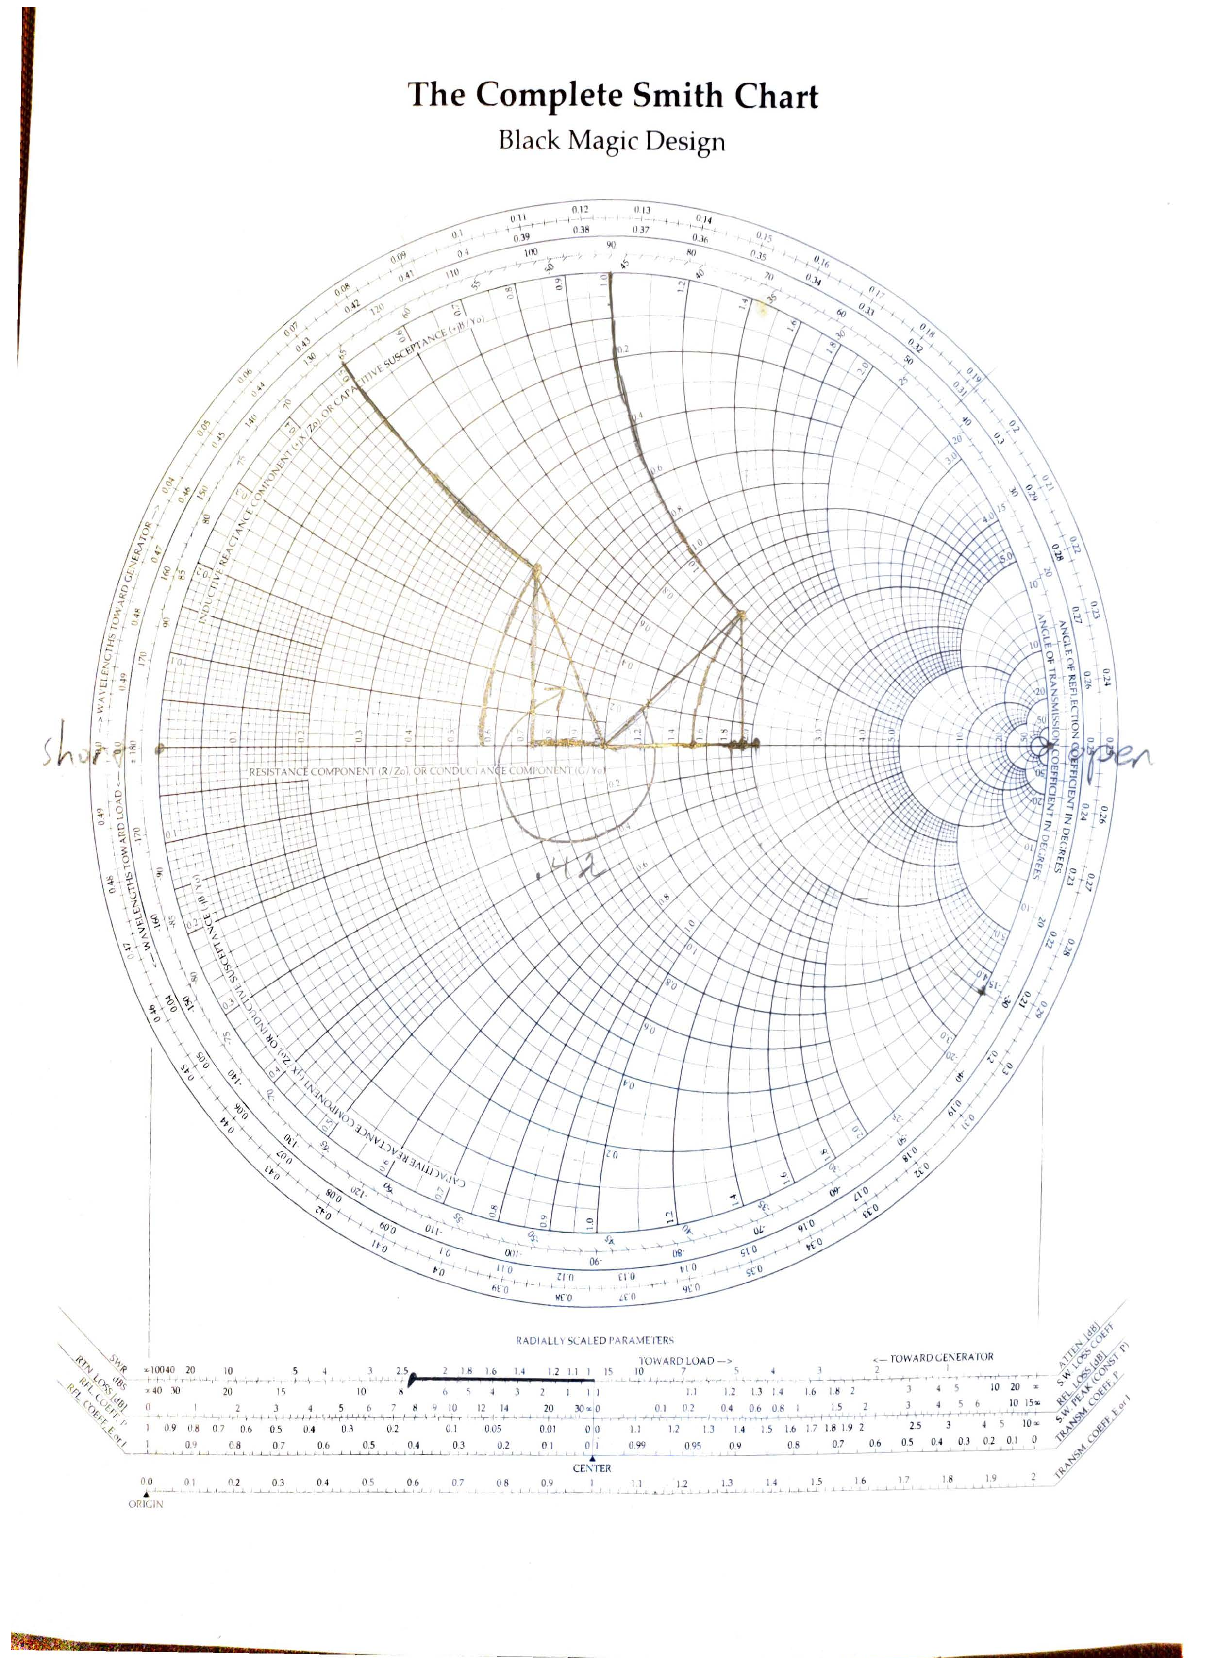
\includepdf[pages=-]{smith_chart.pdf}
\item[1.3]
\ \\
\begin{lstlisting}[language=matlab]
%% ZinSITL: plot Z_in for a simi-infinite transmission line carrying a sinusoid
%
% user specified variables:
%   - Z_0: charcteristic impedance of the line
%   - l: length of the line wavelengths of the transmitted wave
%   - Z_L: load impedance
%
% usage:
% When a user sets the specified inputs, the program produces plots
% of the magnitue and phase of the input impedance of a corresponding
% semi inifinite transmission line up to the desired length.

% user specified inputs
Z_0 = 50; l = 5; Z_L = 10+j20;

% compute Z_in
lVals = 0:l/1000:l;
Z_in = Z_0 * (Z_L + 1j*Z_0*tan(2*pi*lVals)) ./ (Z_0 + 1j*Z_L*tan(2*pi*lVals));

% create plots
figure
subplot(2,1,1)
plot(lVals,abs(Z_in))
ylabel('|Z_{in}|')
subplot(2,1,2)
plot(lVals,angle(Z_in)*180/pi)
ylabel('\angle Z_{in}')
xlabel('\lambda from generator')
\end{lstlisting}
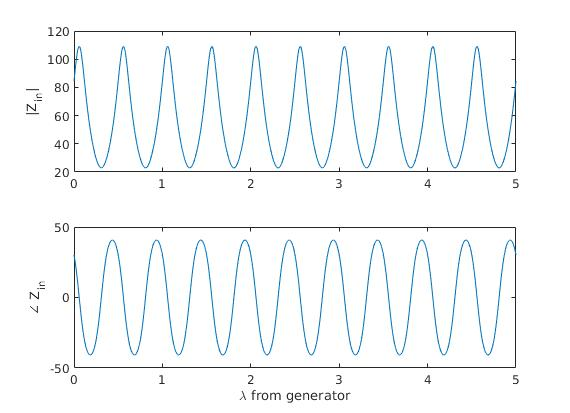
\includegraphics[width=\textwidth]{HW1-3}
\end{enumerate}

\end{document}
